\documentclass{article}
\usepackage[top=0.75in, bottom=0.75in, left=1.25in, right=1in]{geometry} % formatage
\usepackage[frenchb]{babel}
\usepackage[utf8]{inputenc} 
\usepackage{amsmath} % pour utiliser des maths de base 
\usepackage{amssymb} % pour faire \mathcal{}=>des lettres ''cursives''
\usepackage{amsthm} % La petite boîte de fin de preuve
\usepackage{graphicx} % pour importer des images...http://www.tex.ac.uk/cgi-bin/texfaq2html?label=figurehere
\usepackage{titlesec} % automatique, pour faire des sous-titres moins laids
%\usepackage{cancel}
\usepackage[procnames]{listings}
\usepackage[T1]{fontenc}        % http://tex.stackexchange.com/questions/11897/draw-a-diagonal-arrow-across-an-expression-in-a-formula-to-show-that-it-vanishes%
\usepackage[squaren]{SIunits}
\usepackage{subcaption} % Avoir plusieurs sous-figures (graphiques) dans une figures et pouvoire les étiqueter
\usepackage{color}
\usepackage{lipsum}
\usepackage{caption}
\usepackage{enumitem} % Permet d'avoir plus de flexibilité dans les enumerations.
\usepackage{wasysym} 
\usepackage{braket}
\usepackage{mathtools}
\usepackage{multirow} % Fusionner des lignes dans un tableau
\usepackage{mathrsfs} % Faire le symbole de la transformée de Laplace
\usepackage{bbm}
\usepackage{array}
\usepackage{diagbox} % diagonale dans les tableaux
\usepackage{dsfont} % Faire des belles indicatrices                         
\usepackage{float} % placer les tableaux et images où tu veux
\usepackage{listings}
\usepackage[utf8]{inputenc}
\usepackage{comment}
\usepackage{pst-node}
\usepackage{fancyvrb} % Les varbatims gardent l'indentation
\usepackage{enumitem}
\usepackage{breakcites} % Faire en sorte que les citations ne sortent pas dans la marge
\usepackage{graphicx} % Insérer des graphiques
\usepackage{pgfplots}
\usepackage{hyperref} % Faire des hyperliens
\usepackage{verbatim} % Inclure un fichier .text en verbatim
\usepackage{xcolor}
\pgfplotsset{width=10cm, compat=1.9}

% Changer la couleur des hyperliens
\hypersetup{colorlinks = true,
	allcolors  = blue, % default color = black
	%	citecolor  = black
}  


% redefine \VerbatimInput
\RecustomVerbatimCommand{\VerbatimInput}{VerbatimInput}%
{fontsize=\footnotesize,
	%
	frame=lines,  % top and bottom rule only
	framesep=2em, % separation between frame and text
	rulecolor=\color{Gray},
	%
	label=\fbox{\color{Black}data.txt},
	labelposition=topline,
	%
	commandchars=\|\(\), % escape character and argument delimiters for
	% commands within the verbatim
	commentchar=*        % comment character
}


\newcommand{\RomanNumeralCaps}[1]
    {\MakeUppercase{\romannumeral #1}}

\newtheorem{lemme}{Lemme}
\newtheorem{preuve}{Preuve}
\newtheorem{code}{Code informatique}
\newtheorem{exemple}{Exemple}
\newtheorem{scenario}{Scénario}
\newtheorem{algo}{Algorithme}
\newtheorem{definition}{Définition}
\newtheorem{proposition}{Proposition}
\newtheorem{propriete}{Propriété}
\newtheorem{test_hypothese}{Teste d'hypothèse}

\begin{document}
	\renewcommand{\tablename}{Tableau}
	\renewcommand{\figurename}{Illustration}
	
	\begin{titlepage}
		\centering % Centre everything on the title page
		
		\scshape % Use small caps for all text on the title page
		
		\vspace*{7\baselineskip} % White space at the top of the page
		
		%------------------------------------------------
		%	Title
		%------------------------------------------------
		
		\rule{\textwidth}{1.6pt}\vspace*{-\baselineskip}\vspace*{2pt} % Thick horizontal rule
		\rule{\textwidth}{0.4pt} % Thin horizontal rule
		
		\vspace{0.75\baselineskip} % Whitespace above the title
		{\LARGE Travail pratique 1\\} % Title
%		\vspace{0.75\baselineskip}
		\vspace{0.75\baselineskip} % Whitespace below the title
		
		\rule{\textwidth}{0.4pt}\vspace*{-\baselineskip}\vspace{3.2pt} % Thin horizontal rule
		\rule{\textwidth}{1.6pt} % Thick horizontal rule
		
		\vspace{4\baselineskip} % Whitespace after the title block
		
		%------------------------------------------------
		%	Subtitle
		%------------------------------------------------
		
		Travail présenté à \\
		{\scshape\Large M. Thierry Duchesne\\}
		
		\vspace*{4\baselineskip}
		
		Dans le cadre du cours\\
		{\scshape\Large Théorie et applications des méthodes de régression \\ STT-7125}
		
		% Subtitle or further description
		
		\vspace*{4\baselineskip} % Whitespace under the subtitle
		
		%------------------------------------------------
		%	Editor(s)
		%------------------------------------------------
		
		Réalisé par l'équipe 7:\\
		{\scshape\Large Alexandre Lepage\\
		\& Amedeo Zito} % Editor list
		
		\vspace*{5\baselineskip}
		
		le 2 novembre 2020
		
		\vspace{0.4\baselineskip} % Whitespace below the editor list
		
		\vfill % Whitespace between editor names and publisher logo
		
		%------------------------------------------------
		%	Publisher
		%------------------------------------------------
		
		
\includegraphics[height=1.2cm]{UL_P.pdf}\\
		
		Faculté des sciences et de génie\\
		École d'actuariat\\
		Université Laval
		
		\vspace*{3\baselineskip}
		
	\end{titlepage}
	
%	\pagenumbering{Roman} % Pagination en chiffres romains
%	\setcounter{page}{0} 
%	
%	\newpage
%	\strut % Page blanche
%	\newpage
%	
%	\tableofcontents
%	\renewcommand{\listfigurename}{Liste des illustrations}
%	\newpage
%	
%	\listoffigures
%	\listoftables
%	\newpage
%	
%	\pagenumbering{arabic} % Pagination en chiffres normaux
%	\setcounter{page}{1}


\section{Introduction}
Les méthodes de régression linéaires sont fort utiles afin d'identifier des variables pouvant expliquer un comportement ou un phénomène et elles peuvent s'avérer efficaces pour faire de la prédiction si les données disponibles sont appropriées.\\

L'objet de ce travail est d'expérimenter l'utilisation de cette famille de modèles afin de résoudre trois problèmes de nature différente. 
%
La premier d'entre eux consiste à réaliser une régression linéaire afin de prédire le taux de mortalité à partir de variables mesurant la pollution environnementale et les caractéristiques socio-démographiques de 60 localités.
%
Le second problème consiste à construire un modèle de régression qui estime
la probabilité de diagnostic de maladie coronarienne. L'objectif étant de définir les facteurs associés à une hausse du risque d’un diagnostic positif de maladie coronarienne.
%
En ce qui a trait au dernier problème, celui-ci s'inscrit dans un contexte d'assurance automobile et consiste à construire un modèle afin de voir s’il y a une association entre les caractéristiques du véhicule et de l'assuré et le nombre de réclamations.

\section{Analyse et traitement de la multicollinéarité}\label{sect_multicollinearite}
La force des modèles de régression linéaire provient de l'hypothèse que la matrice de schéma $\boldsymbol{X}$ est de plein rang; c.-à-d. qu'aucune colonne n'est linéairement dépendante des autres colonnes. Ce faisant, on s'assure qu'il n'existe qu'un seul inverse possible à la matrice $\boldsymbol{X}'\boldsymbol{X}$; de ce fait, on s'assure également que le vecteur des paramètres du modèle $\hat{\boldsymbol{\beta}}$ soit unique (un seul minimum à la fonction de perte utilisé pour l'entraînement). Ainsi, s'il existe un problème de multicolinéarité, il en découlerait que la matrice de schéma $\boldsymbol{X}$ ne serait plus de plein rang et il pourrait exister plusieurs minimum locaux à la fonction de perte utilisée pour entraîner le modèle. Il en résulterait alors une instabilité dans la convergence des paramètres et la variance de certaines de ces composantes serait démesurément grande.
%
Pour cette raison, avant même de réaliser la sélection de modèle pour chacune des étapes, il faut d'abord mesurer le degré de multicollinéarité entre les potentielles variables explicatives disponibles.\\

Un outil bien pratique pour détecter la présence de multicollinéarité est le facteur d’inflation de la variance (VIF). Ce dernier peut être calculé avec la fonction \texttt{ols\_vif\_tol()} du \textit{package} \texttt{olsrr} en \texttt{R}. Cependant, si les données utilisées comportent une ou plusieurs variables catégorielles, cette mesure n'est plus adéquate (voir \cite{fox1992generalized}). Dans ce cas, on préférera le facteur d'inflation généralisé (GVIF) et sa version standardisée: $(\mathrm{GVIF}_j)^{1/(2 p_j)}$ , où $p_j$ correspond au nombre de degrés de libertés (le nombre de paramètres) rattachés à la $j^\mathrm{e}$ variable explicative du modèle, $j\in \{1,\dots,p'\}$. 
À noter que lorsque $p_j=1$, alors $\mathrm{GVIF}_j = \mathrm{VIF}_j$.
%
Afin de mesurer cette métrique, Fox et Monette ont créé la fonction \texttt{vif} du \textit{package} \texttt{car}. De façon générale, plusieurs auteurs suggèrent de considérer que $\mathrm{VIF_j}>10$ pourrait signaler un problème de multicolinéarité. En suivant cette logique, on peut considérer qu'il y a problème de multicolinéarité si $(\mathrm{GVIF}_j)^{1/(2 p_j)} > \sqrt{10} \approx 3.16,$ pour $j=1,\dots,p'$.\\

Si, effectivement, un problème de multicolinéarité est détecté, alors la fonction \texttt{ols\_eigen\_cindex()} du \textit{package} \texttt{olsrr} permet de faire un diagnostique plus approfondi. En effet, cette fonction permet de calculer les valeurs propres (\textit{eigen values}) associées à la matrice des coefficients de corrélation échantillonnaux $\boldsymbol{X^{\star}}'\boldsymbol{X^{\star}}$. 
%
À partir de celles-ci, elle calcule des indices de conditionnement définis comme
$$\phi_j = \sqrt{\frac{\lambda_{max}}{\lambda_j}},\ j=1,\dots,p',$$
où $\lambda_j$ correspond à la $j$-ème valeur propre de $\boldsymbol{X^{\star}}'\boldsymbol{X^{\star}}$ et $\lambda_{max}=\max(\lambda_1,\dots,\lambda_{p'}).$
Ces indices de conditionnement sont des indicateurs de la force de dépendance linéaire unissant certaines variables.
%
Ainsi, on regardera la ligne du tableau correspondant à la valeur de $\phi_j$ qui est la plus élevée. Une règle du pousse veut que si $\phi_j > 30$, alors on est en présence de multicolinéarité. Dans ce cas, on considérera la  proportion de la variance de $\hat{\beta}_l$ qui est expliquée par la $j$-ème dépendance linéaire, pour $l=1,\dots,p'$. C.-à-d. 
$$ p_{lj} = \frac{v_{lj}^2/\lambda_j}{c_{jj}},$$
où $v_{lj}$ correspond au $l$-ème élément du vecteur propre $\boldsymbol{v}_j$ associé à la $j$-ème valeur propre $\lambda_j$ et $c_{jj} = \sum_{l=1}^{p'}v_{lj}^2/\lambda_j$. 
Si $p_{lj} > 0.6$, alors on conclu que la $l$-ème variable explicative contribue à la $j^\mathrm{e}$ multicolinéarité et cause problème.\\

Dans ce cas, les solutions possibles consistent à appliquer une transformation non linéaire sur les variables explicatives (p.ex. transformation logarithmique ou racine carrée), réduire la dimension de la matrice de schéma en retirant la variable la plus problématique. S'il y a plusieurs valeurs de $l$ pour lesquelles $p_{lj}>0.5$ pour un même $j$, alors il est possible de les regrouper à l'aide d'une moyenne. Par exemple, pour $j=\underset{j\in\{1,\dots,p'\}}{\mathrm{argmax}}\{\phi_j\}$, si on a $p_{1j}>0.5$ et $p_{2j}>0.5$, alors on peut combiner $x_1$ et $x_2$ de la façon suivante: $(x_1+x_2)/2$.\\

Après avoir réalisé ces étapes, il faut recommencer itérativement ce processus jusqu'à ce qu'il n'y ait plus de problème soulevé par l'analyse du VIF ou du GVIF.


\section{Question 1}

	Pour la première question de ce travail, on considère un jeu de données présentant des variables mesurant la pollution environnementale et les caractéristiques socio-démographiques de 60 localités. L'objectif de cette question est de valider qu'il est possible de prédire la mortalité d'une région en fonction de ces variables explicatives et de donner un estimé ponctuel ainsi qu’un intervalle de confiance à 95\% sur une observation de donnée.
	
	\subsection{Traitement de la multicollinéarité}
	
	Pour atteindre cet objectif, la première étape consiste à réaliser une analyse de multicollinéarité telle que décrite dans la section \ref{sect_multicollinearite}. Se faisant, on découvre que les VIFs pour les variables A12 et A13 sont supérieures à 10. Afin de traiter ce problème, on peut commencer par regarder s'il est pertinent d'effectuer une transformation non linéaire de certaines variables explicatives. Afin de visualiser les options envisageable, les illustrations \ref{Qst1_transformations_1} à \ref{Qst1_transformations_5} présentent l'effet d'une transformation logarithmique (au centre) et celui d'une transformation racine carrée (à droite) sur la relation existant entre la variable endogène et chacune des variables explicatives. Si on voit que cette transformation améliore la relation de linéarité existant entre les variables en question, alors on procède à la transformation appropriée. Suite à l'analyse des illustrations \ref{Qst1_transformations_1} à \ref{Qst1_transformations_5}, on en vient à considérer que les variables A12 et A13 méritent à recevoir une transformation logarithmique, de même que les variables A9 et A14 profiterait à recevoir une transformation racine carrée. Afin de valider ces observations, on teste différents modèles utilisant plusieurs combinaisons de transformations. Il advient que le modèle complet possédant l'AIC le plus petit est le suivant:
	\begin{align}\label{modele_complet}
		\mathrm{B} &\sim \mathrm{A1 + A2 + A3 + A4 + A5 + A6 + A7 + A8 + I(sqrt(A9))}\\
			&\mathrm{+ A10 + A11 + I(log(A12)) + I(log(A13)) + I(log(A14)) + A15}.\nonumber
	\end{align}
	
	Une fois que ces transformations sont effectuées, on refait l'analyse des VIFs. Puisque celle-ci nous indique que la multicollinéarité n'est toujours pas réglée, on procède aux étapes décrites dans la section \ref{sect_multicollinearite} après quoi on trouve le modèle suivant:
	\begin{equation}\label{modele_traitement_multicol_methode_iterative}
		\mathrm{B} \sim \mathrm{A1 + A2 + A8 + A11 + I(log(A14)) + I(log(sqrt(A12 * A13)))}.
	\end{equation}
	
	À titre comparatif, nous avons voulu tester s'il était possible d'avoir un modèle plus performant si le traitement de la multicolinéarité était fait par sélection de variables en utilisant une régression LASSO. Avec la fonction \texttt{glm.net} du \textit{package} du même nom et avec le paramètre \texttt{alpha=1}, on essaie plusieurs valeurs pour le terme de pénalité $\lambda$ en commençant par celui qui est le plus inclusif (lambda le plus petit). Ainsi, on trouve que la valeur de $\lambda$ qui est minimal tout en minimisant la statistique de déviance et en éliminant la multicolinéarité est $\lambda = 5.98761443432345.$ Avec ce dernier, on trouve le modèle suivant:
	\begin{equation}\label{modele_traitement_multicol_methode_LASSO}
		\mathrm{B} \sim \mathrm{A1 + A2 + A6 + A7 + A8 + I(log(A13)) + I(log(A14)) + I(sqrt(A9))}.
	\end{equation}
	Ainsi, si on compare les modèles \eqref{modele_traitement_multicol_methode_iterative} et \eqref{modele_traitement_multicol_methode_LASSO}, on trouve que le modèle \eqref{modele_traitement_multicol_methode_LASSO} est celui qui minimise l'AIC et qui maximise également la statistique du $R^2$ de prédiction. Conséquemment, il s'agira du modèle de base utilisé pour la sélection des variables.
	
	\subsection{Sélection des variables explicatives}
	On se rappelle que l'objectif de cette question est de construire un modèle prédictif. Conséquemment, pour se faire, l'idéal est de produire tous les sous-modèles possibles découlant de \eqref{modele_traitement_multicol_methode_LASSO}.
	Cette opération peut être réalisée avec la fonction \texttt{ols\_step\_all\_possible} du \textit{package} \texttt{olsrr}. Une fois que tous les sous-modèles sont produits, on regarde les 3 modèles qui maximisent la statistique du $R^2$ de prédiction comme le démontre l'illustration \ref{Qst1_all_possible_models_top3}.
	\begin{figure}[H]
		\centering
		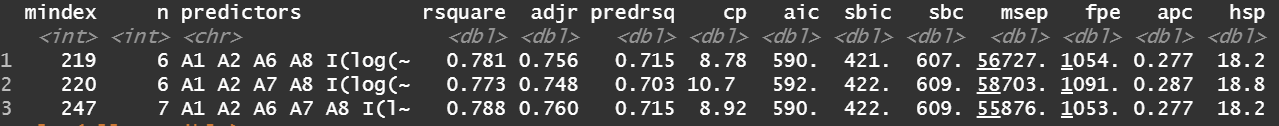
\includegraphics[width=\textwidth]{graphiques/Qst1_all_possible_models_top3}
		\caption{Résultats des trois meilleurs modèles selon la statistique du $R^2$ de prédiction.}
		\label{Qst1_all_possible_models_top3}
	\end{figure}
	Comme les modèles 219 et 247 sont très comparables, on choisira celui qui est le plus simple étant donné que le jeu de données d'entraînement comporte très peu d'observations (60). Conséquemment, le modèle sélectionné est le suivant:
	\begin{equation}\label{modele_variables_selectionnees}
		\mathrm{B} \sim \mathrm{A1 + A2 + A6 + A8 + I(log(A13)) + I(sqrt(A9))}.
	\end{equation}
	À ce stade, il pourrait être intéressant d'observer des interactions entre ces variables. Pour identifier celles qui sont d'intérêt, on applique le test F partiel sur toutes les interactions de 1er ordre possible. Se faisant, on trouve qu'aucune des interactions n'est significative au seuil de 1\%. Donc, le modèle \eqref{modele_variables_selectionnees} correspond à notre modèle final.\\
	
	Avec la fonction \texttt{ols\_regress} du \textit{package} \texttt{olsrr}, on peut calculer plusieurs statistiques d'intérêt pour décrire celui-ci. D'une part, on a un $R^2$ de prédiction qui est de 71\%, ce qui est très bon considérant que la mortalité est un phénomène complexe auquel il est impossible de décrire à 100\% avec des variables explicatives. D'autre part, la statistique de Wald nous indique que chacune des variables explicatives incluses dans le modèle est significative à un seuil de 5\%.
	
	\subsection{Calcule de la prédiction}
	Maintenant que l'on a un modèle appréciable, on aimerait calculer un estimé ponctuel ainsi qu’un intervalle de confiance à 95\% pour le taux de mortalité à un endroit pour lequel les variables A1 à A15 valent respectivement
	\begin{center}
		40 30 80 9 3 10 77 4100 13 46 15 25 26 145 55.
	\end{center}
	Avec la fonction \texttt{predict} du \textit{package} \texttt{stats}, on obtient un estimé de $\hat{B} = 999.4799$ ainsi qu'un intervalle de prédiction correspondant à  $B \in [936.0751, 1062.885]$.
	
\section{Question 2}
 
	\appendix
	\section{Illustrations}
	\begin{figure}[H]
		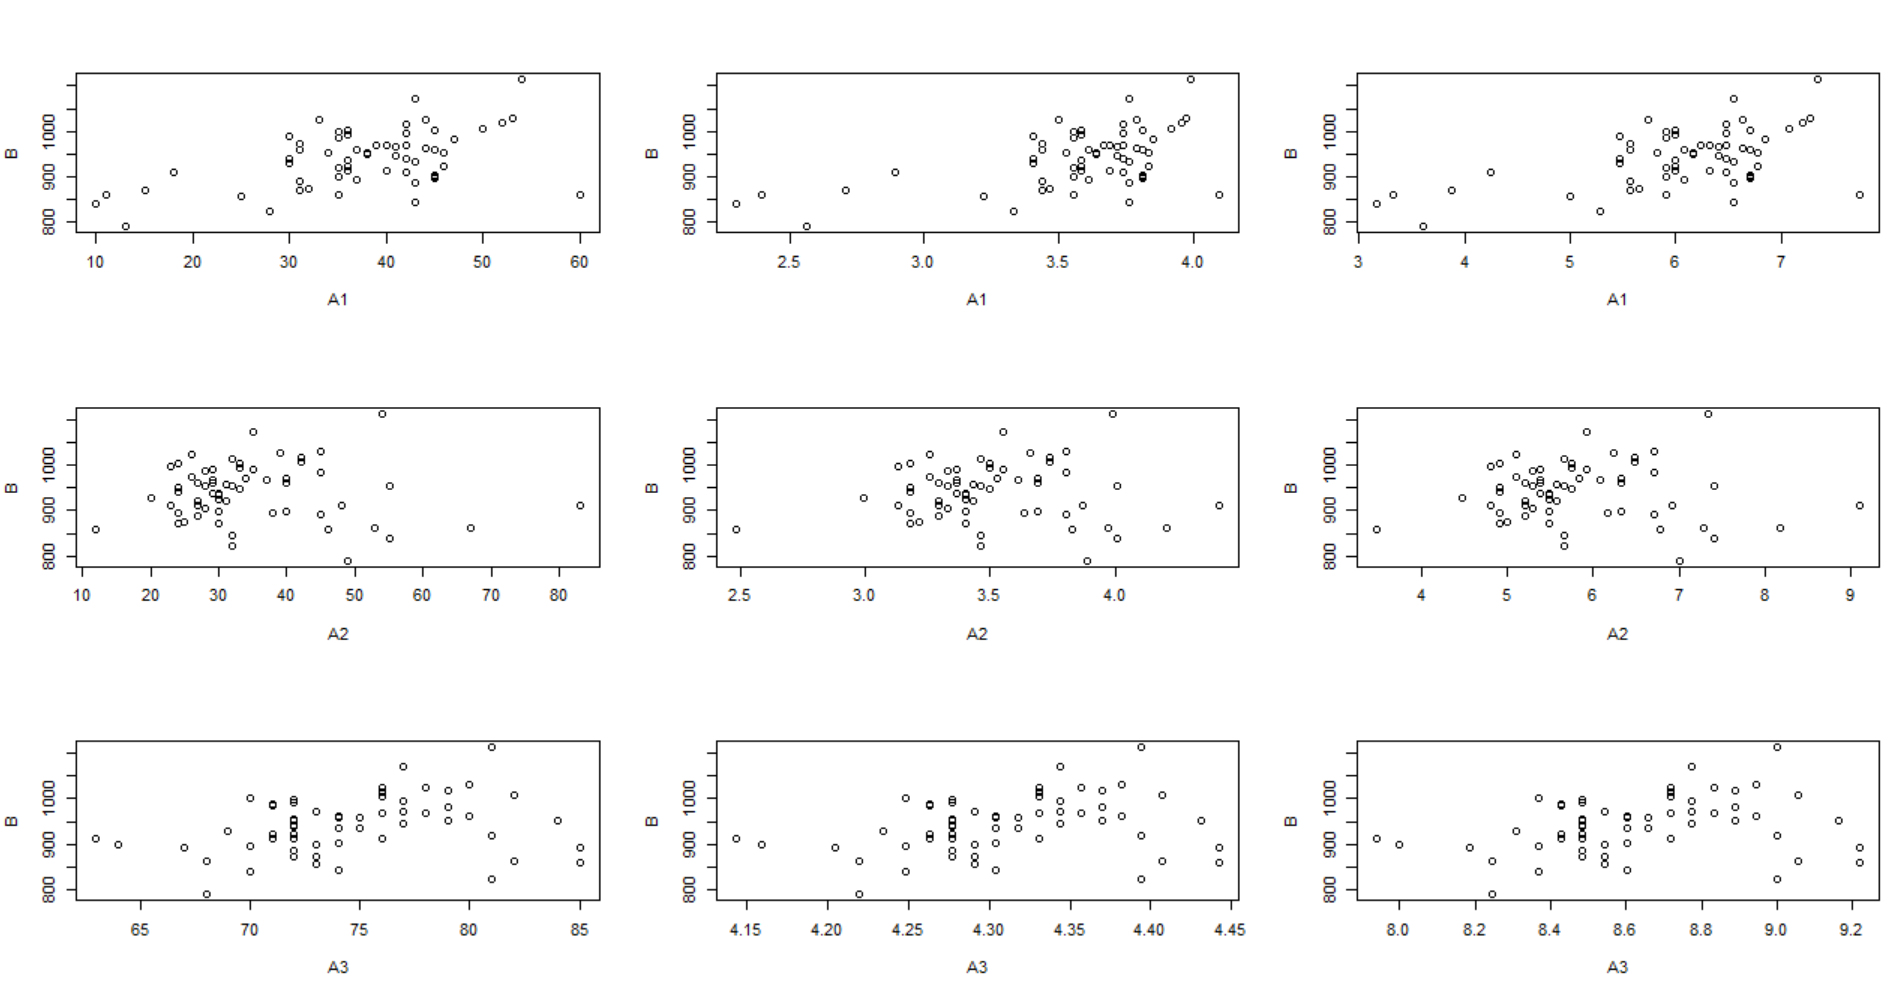
\includegraphics[width=\textwidth]{graphiques/Qst1_transformations_1}
		\caption{À gauche, on compare la variable endogène B avec les variables exogènes A1 à A3. Au centre, on compare la même relation, mais avec une transformation logarithmique effectuée sur les variables exogènes. À droite, c'est la transformation racine carrée qui est appliquée.}
		\label{Qst1_transformations_1}
	\end{figure}
	\begin{figure}[H]
		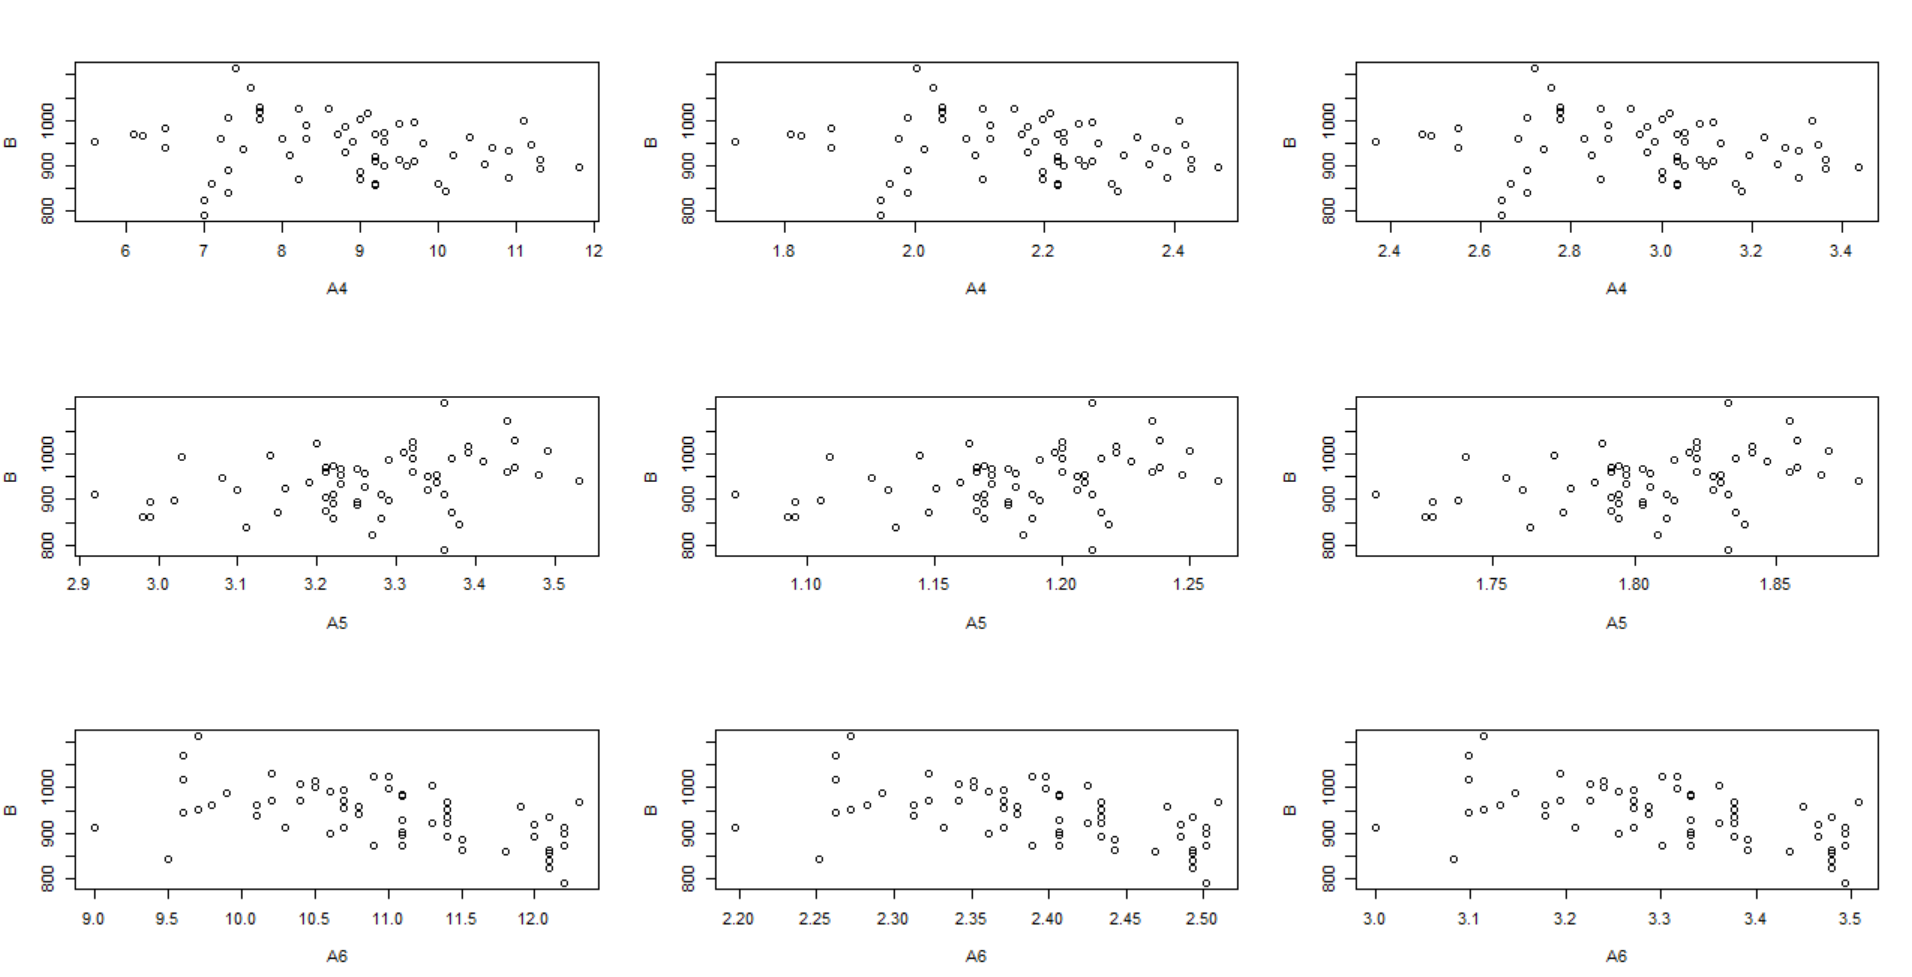
\includegraphics[width=\textwidth]{graphiques/Qst1_transformations_2}
		\caption{À gauche, on compare la variable endogène B avec les variables exogènes A4 à A6. Au centre, on compare la même relation, mais avec une transformation logarithmique effectuée sur les variables exogènes. À droite, c'est la transformation racine carrée qui est appliquée.}
		\label{Qst1_transformations_2}
	\end{figure}
	\begin{figure}[H]
		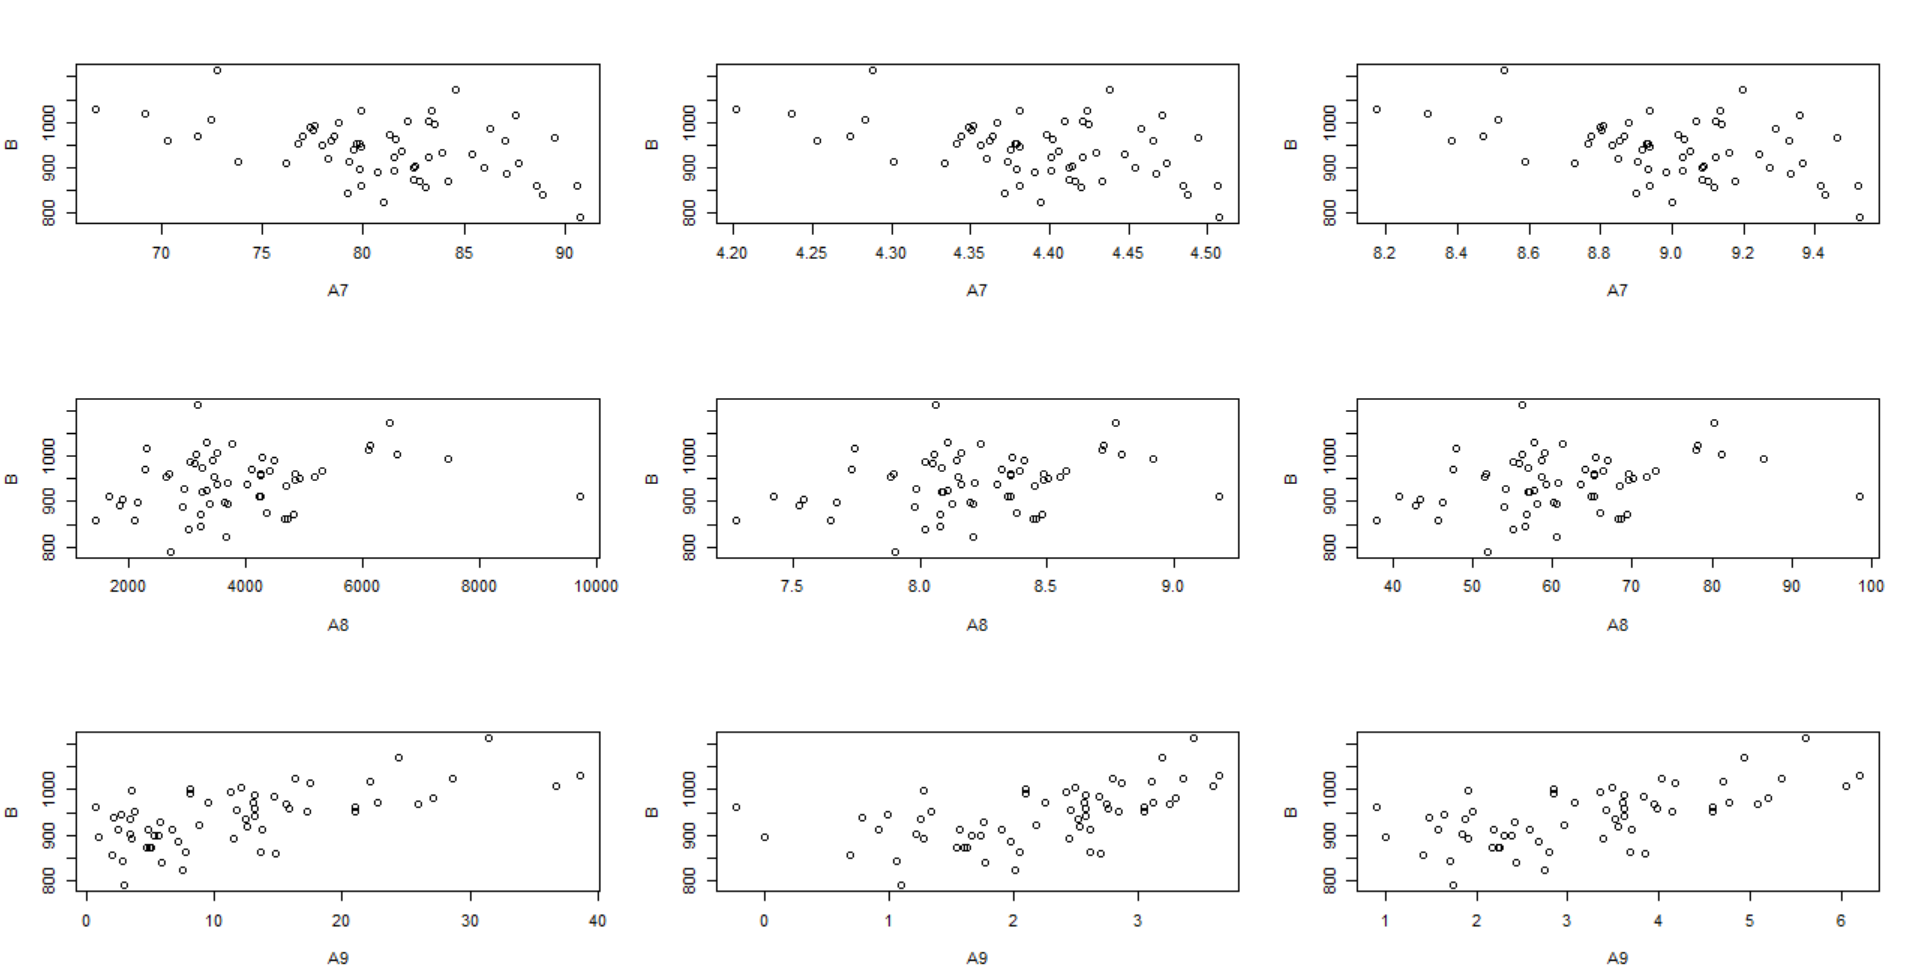
\includegraphics[width=\textwidth]{graphiques/Qst1_transformations_3}
		\caption{À gauche, on compare la variable endogène B avec les variables exogènes A7 à A9. Au centre, on compare la même relation, mais avec une transformation logarithmique effectuée sur les variables exogènes. À droite, c'est la transformation racine carrée qui est appliquée.}
		\label{Qst1_transformations_3}
	\end{figure}
	\begin{figure}[H]
		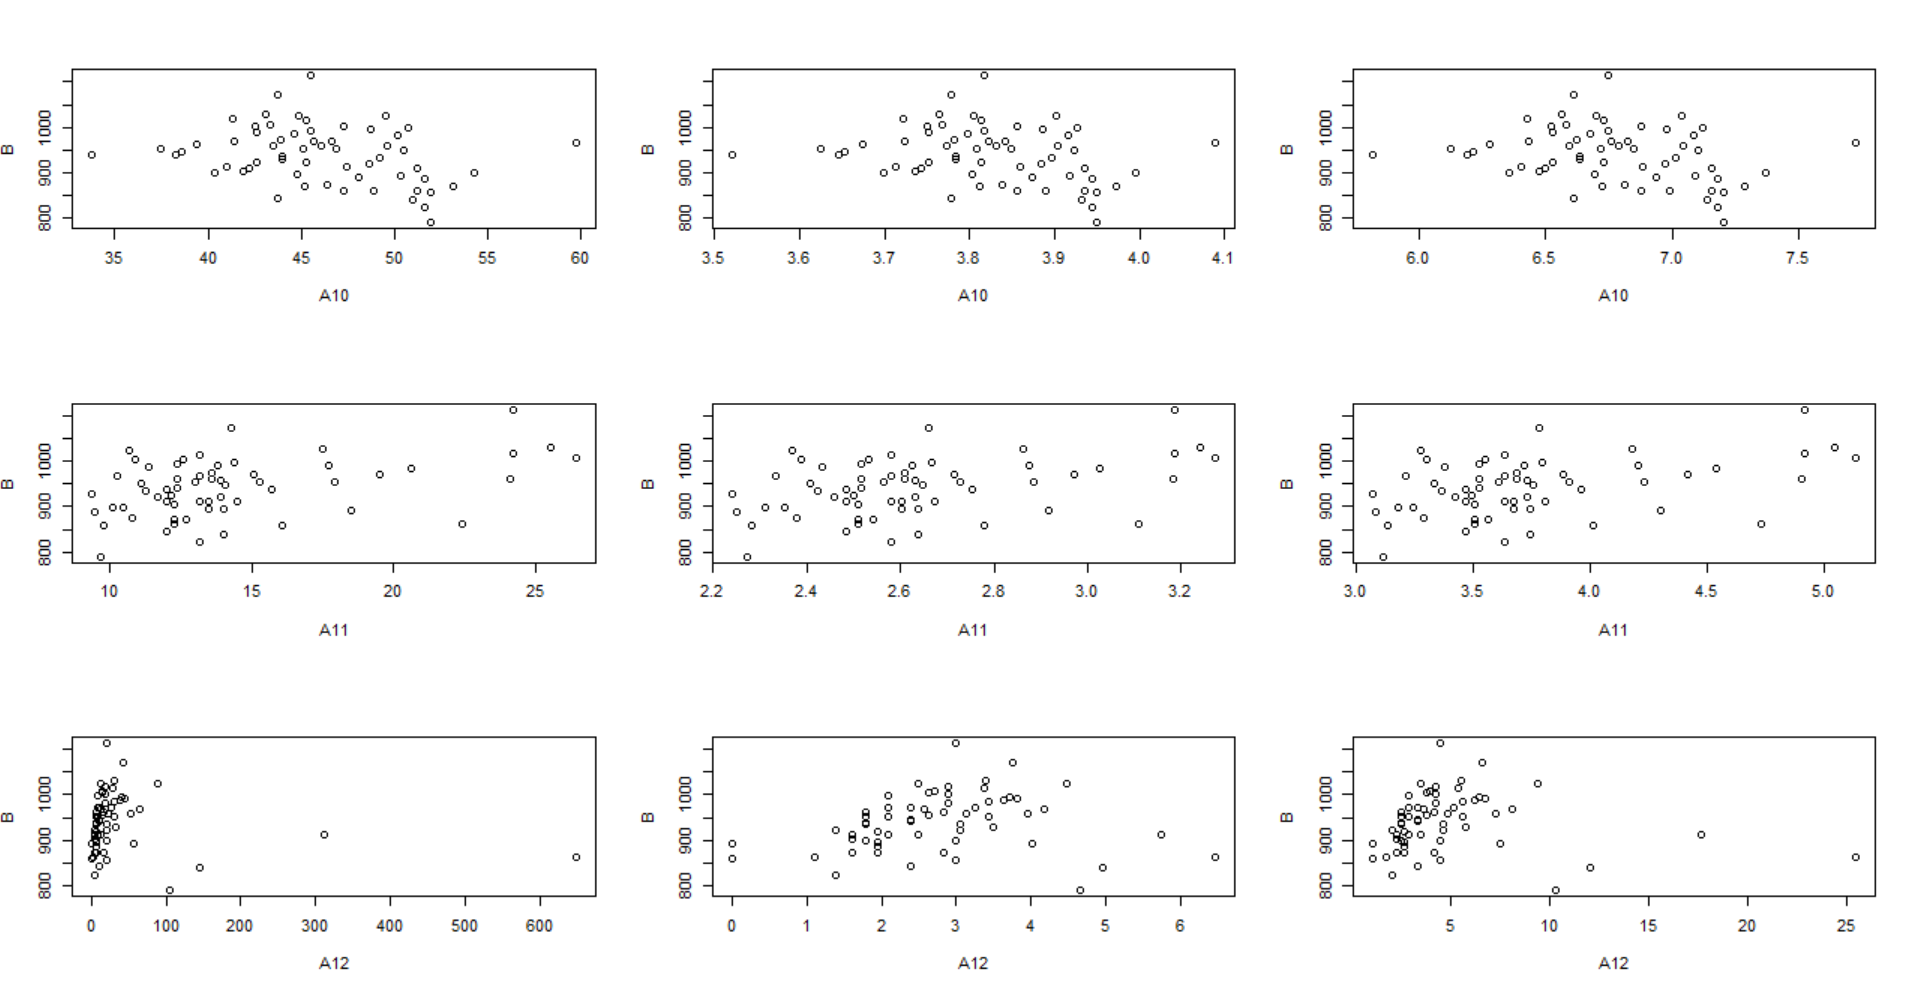
\includegraphics[width=\textwidth]{graphiques/Qst1_transformations_4}
		\caption{À gauche, on compare la variable endogène B avec les variables exogènes A10 à A12. Au centre, on compare la même relation, mais avec une transformation logarithmique effectuée sur les variables exogènes. À droite, c'est la transformation racine carrée qui est appliquée.}
		\label{Qst1_transformations_4}
	\end{figure}
	\begin{figure}[H]
		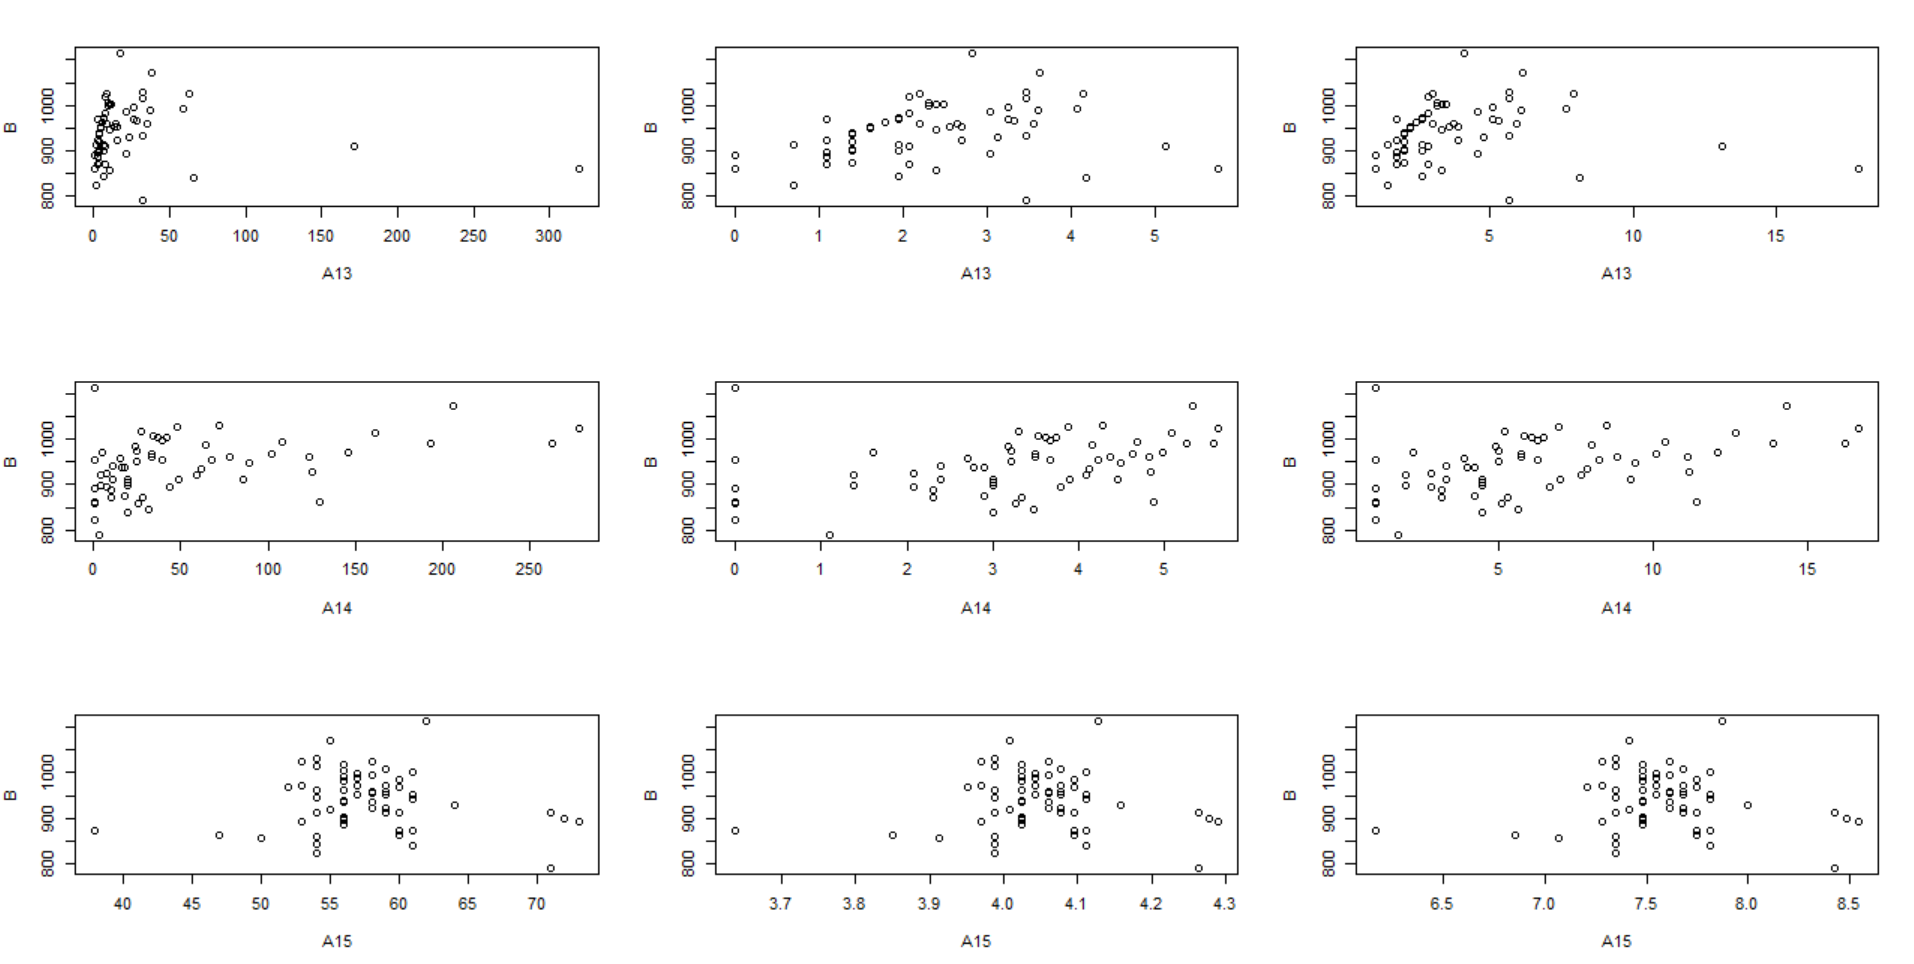
\includegraphics[width=\textwidth]{graphiques/Qst1_transformations_5}
		\caption{À gauche, on compare la variable endogène B avec les variables exogènes A13 à A15. Au centre, on compare la même relation, mais avec une transformation logarithmique effectuée sur les variables exogènes. À droite, c'est la transformation racine carrée qui est appliquée.}
		\label{Qst1_transformations_5}
	\end{figure}
	
	\clearpage
	\bibliographystyle{apalike}
	\bibliography{BibGLM}	
	
\end{document}